
%\documentclass[manuscript]{acmart}
%\documentclass[acmsmall]{acmart}
%\settopmatter{printacmref=false}


\documentclass[
  a4paper,
  12pt,
  DIV=12,        % höherer Wert = schmalere Ränder, weniger Whitespacmi
  parskip=half,  % Absätze mit halbem Abstand statt Einzug
  headings=small % kleinere Überschriften, weniger vertikaler Abstand
]{scrartcl}

%\documentclass[a4paper,11pt]{scrartcl}
%\documentclass[a4paper,11pt]{report}
%\documentclass[a4paper,12pt]{book}
\usepackage[utf8]{inputenc}
\usepackage[german]{babel}
\usepackage[T1]{fontenc}
\usepackage{lmodern}
\usepackage[inkscapelatex=false]{svg}
% Texte im SVG von Inkscape setzen lassen, nicht durch die Dokumentschrift ersetzen
\svgsetup{inkscapelatex=false}
\usepackage{amsmath}
\usepackage{caption}
\usepackage{gensymb}
\usepackage{microtype}
\usepackage{longtable}
\usepackage{tabularx}   % Spalten, die die restliche Zeilenbreite auffüllen (X-Spalte)
\usepackage{booktabs}   % \toprule \midrule \bottomrule (in mobrob_table.tex verwendet)
\usepackage{wrapfig}    % Textumfluss um Abbildungen
\usepackage{array}
\usepackage{calc}

\usepackage[citecolor=black, colorlinks=true, linkcolor=black, urlcolor=blue]{hyperref}


%\usepackage{geometry}
\usepackage{siunitx}
%\geometry{margin=2.5cm}


\usepackage{amsthm}
\usepackage{mdframed}
\usepackage{enumitem}

\newmdtheoremenv{theorem}{Theorem}

\theoremstyle{definition}
\newmdtheoremenv{derivation}{Derivation}

\providecommand{\tightlist}{%
  \setlength{\itemsep}{0pt}\setlength{\parskip}{0pt}}

%\mdfdefinestyle{leftline}{
%    topline=false, bottomline=false, rightline=false,
%    linewidth=2pt, linecolor=gray
%}
\theoremstyle{definition}
\newmdtheoremenv[style=leftline]{myalgorithm}{Algorithm}




%\usepackage{fancyvrb}







\let\Bbbk\relax
\usepackage{amssymb}


\usepackage{yfonts}

\usepackage{kvmap}

\usepackage[
    backend=biber,
    style=alphabetic,
    sortlocale=de_DE,
    natbib=true,
    %url=false,
    doi=true,
    %eprint=false
]{biblatex}
% \addbibresource{Literaturrecherche-Stefan-Etringer/algo-references.bib}

%\usepackage[
%    backend=biber,
%    style=alphabetic,
%    sortlocale=de_DE,
%    natbib=true,
%    %url=false,
%    doi=true,
%    %eprint=false
%]{biblatex}
%\addbibresource{Literaturrecherche-Dennis/mobrob_references.bib}

\usepackage[autostyle=true,german=quotes]{csquotes}
\usepackage{trfsigns} %fourier transform arrow
\usepackage{mathrsfs} %fourier F
\usepackage{commath}

\usepackage{pgfplots}
\pgfplotsset{compat=1.18}

\usepackage{xcolor}
\usepackage{listings}
\usepackage[european]{circuitikz}
\ctikzset{tripoles/european not symbol=ieee circle}

%\usepackage[shading]{moeptikz}
%\moeptikzset{shading=true}

%\usepackage{german,longtable}

\usepackage{xcolor}
\usepackage{color}
\usepackage{url}

\usepackage{xfrac}

\usepackage{listings}
\usepackage{verbatimbox}

\usepackage{algorithm}
\usepackage{algpseudocode}

\usepackage{multirow}
\usepackage{float}
\usepackage{pdflscape}   % einzelne Querformatseiten (im PDF gedreht)

%%%% TIKZ

\usepackage{tikz}

\usepackage{pgfplots}
\usetikzlibrary{calc,
trees,positioning,arrows,
chains,shapes.geometric,
decorations.pathreplacing,
decorations.pathmorphing,shapes,
matrix,shapes.symbols,
plotmarks}
%\tikzexternalize[prefix=figures/]

%\tikzset{%
%  block/.style    = {draw, thick, rectangle, minimum height = 3em,
%    minimum width = 3em},
%  sum/.style      = {draw, circle, node distance = 2cm}, % Adder
%  input/.style    = {coordinate}, % Input
%  output/.style   = {coordinate} % Output
%}
% Defining string as labels of certain blocks.
%\newcommand{\suma}{\Large$+$}
%\newcommand{\multa}{\Large$\times$}
%\newcommand{\inte}{$\displaystyle \int$}
%\newcommand{\derv}{\huge$\frac{d}{dt}$}

\usetikzlibrary{arrows,automata,positioning}
%\usepackage{automata}


%%% END TIKZ

\usepackage[section]{placeins}

\usepackage{textcomp}


\usepackage{listings}
\usepackage{verbatimbox}

\usepackage{bold-extra}

\usepackage{framed}

%\usepackage{fancyhdr}
%\pagestyle{fancy}
%\lhead{\leftmark}
%\chead{}
%\rhead{}
%\lfoot{}
%\cfoot{\thepage}
%\rfoot{}
%\renewcommand{\headrulewidth}{0.2pt}
%\renewcommand{\footrulewidth}{0.2pt}



\newcommand{\Z}{\mathbb{Z}}
\newcommand{\R}{\mathbb{R}}
\newcommand{\C}{\mathbb{C}}
\newcommand{\N}{\mathbb{N}}
\newcommand{\SqrtNy}{$\sqrt{\textsc{Ny}}$}
\newcommand{\conj}{\overline}
\newcommand{\Kset}{\textswab{K}}
\newcommand{\Qset}{\textswab{Q}}
\newcommand{\ceil}[1]{\left\lceil #1 \right\rceil}
\newcommand{\floor}[1]{\left\lfloor #1 \right\rfloor}
\newcommand{\sorted}[1]{\textsc{sort}\left\lbrace #1 \right\rbrace}
\newcommand{\SNRgain}{a_{SNR}}
\newcommand{\EQgain}{a_{EQ}}
\newcommand{\SIRgain}{a_{SIR}}
\newcommand{\SNIRgain}{a_{SINR}}
\newcommand{\SNR}{\textsc{SNR}}
\newcommand{\CIRgain}{a_{CIR}}
\newcommand{\CINRgain}{a_{CINR}}
\newcommand{\CNR}{\textsc{CNR}}
\newcommand{\CINR}{\textsc{CINR}}
\newcommand{\HPAModel}{ Hughes 1177H TWTA }
\newcommand{\bigO}{\mathcal{O}}
\newcommand{\CopWinCompl}{2.375377}
\newcommand{\IBO}{\textsc{IBO}}
\newcommand{\OBO}{\textsc{OBO}}
\newcommand{\spacepage}{\newpage\null\thispagestyle{empty}\newpage}
\newcommand{\satcom}{ SatCom }
\newcommand{\db}{~\text{dB}}


\definecolor{mGreen}{rgb}{0,0.6,0}
\definecolor{mGray}{rgb}{0.5,0.5,0.5}
\definecolor{mPurple}{rgb}{0.58,0,0.82}
\definecolor{backgroundColour}{rgb}{0.95,0.95,0.92}

\lstdefinestyle{CStyle}{
    backgroundcolor=\color{backgroundColour},
    commentstyle=\color{mGreen},
    keywordstyle=\color{magenta},
    numberstyle=\tiny\color{mGray},
    stringstyle=\color{mPurple},
    basicstyle=\footnotesize,
    breakatwhitespace=false,
    breaklines=true,
    captionpos=b,
    keepspaces=true,
    numbers=left,
    numbersep=5pt,
    showspaces=false,
    showstringspaces=false,
    showtabs=false,
    tabsize=2,
    language=C
}

\lstdefinelanguage{VHDL}{
  morekeywords=[1]{library,use,all,entity,is,port,in,out,end,architecture,of,begin,process,if,then,else,elsif,when,others,signal,variable,wait,for,loop},
  morecomment=[l]--,
  morestring=[b]",
  sensitive=true
}

\lstset{
  language=VHDL,
  basicstyle=\ttfamily\small,
  keywordstyle=\color{blue},
  commentstyle=\color{gray},
  stringstyle=\color{red},
  numbers=left,
  numberstyle=\tiny,
  stepnumber=1,
  numbersep=8pt,
  frame=single,
  breaklines=true,
  captionpos=b
}

\lstset{numbers=none}

%\newcounter{example}
%\renewcommand{\theexample}{\thesection.\arabic{example}}


% Default fixed font does not support bold face
\DeclareFixedFont{\ttb}{T1}{txtt}{bx}{n}{12} % for bold
\DeclareFixedFont{\ttm}{T1}{txtt}{m}{n}{12}  % for normal

% Custom colors
\usepackage{color}
\definecolor{deepblue}{rgb}{0,0,0.5}
\definecolor{deepred}{rgb}{0.6,0,0}
\definecolor{deepgreen}{rgb}{0,0.5,0}

\usepackage{listings}

% Python style for highlighting
\newcommand\pythonstyle{\lstset{
language=Python,
basicstyle=\ttm,
morekeywords={self},              % Add keywords here
keywordstyle=\ttb\color{deepblue},
emph={MyClass,__init__},          % Custom highlighting
emphstyle=\ttb\color{deepred},    % Custom highlighting style
stringstyle=\color{deepgreen},
frame=tb,                         % Any extra options here
showstringspaces=false
}}


% Python environment
\lstnewenvironment{python}[1][]
{
\pythonstyle
\lstset{#1}
}
{}

% Python for external files
\newcommand\pythonexternal[2][]{{
\pythonstyle
\lstinputlisting[#1]{#2}}}

% Python for inline
\newcommand\pythoninline[1]{{\pythonstyle\lstinline!#1!}}


% ---------------------------------------------------------------------
% Stil fuer C++-Listings dieser Dokumentation
% ---------------------------------------------------------------------
\lstdefinestyle{cpp}{
  language=C++,
  basicstyle=\ttfamily\footnotesize,
  keywordstyle=\color{deepblue},
  commentstyle=\color{mGreen},
  stringstyle=\color{mPurple},
  numbers=none,
  breaklines=true,
  showstringspaces=false,
  frame=single,
  columns=fullflexible,
  captionpos=b
}



%\nocite{*}


\begin{document}
%\pagenumbering{roman}



\title{Coasterbot}
\subtitle{Testreport}
\author{Stefan Etringer}
%\email{gereonsuch@suchdsp.com}
%\affiliation{
%  \institution{Wilhelm Büchner University of Applied Sciences}
%  \department{Computer Engineering}
%  \city{Hof}
%  \country{Germany}
%}



\begin{titlepage}
  \begin{center}
    {\large Wilhelm Büchner University of Applied Sciences} \\[0.3em]

    {\normalsize Projektseminar Master}
\vspace{5em}

    {\LARGE\bfseries Coasterbot} \\[0.5em]

    {\large Testreport} \\[1em]

    {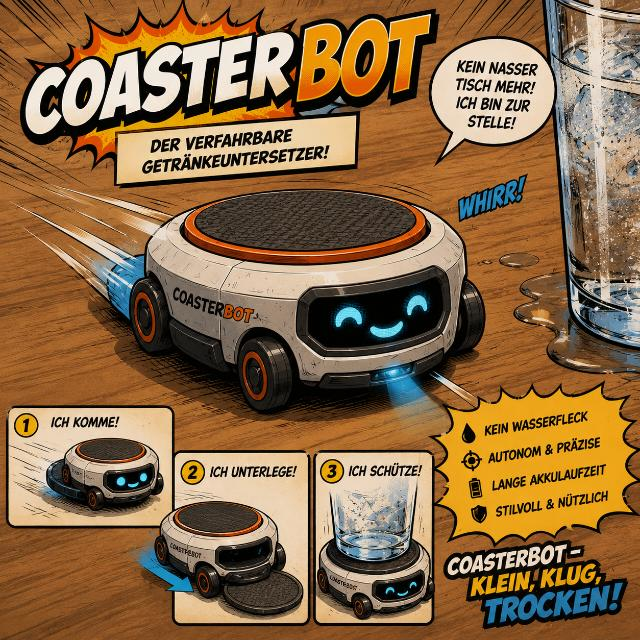
\includegraphics[width=0.38\textwidth]{coasterbot.png}} \\[1em]

\vspace{4em}

    {\normalsize
\begin{tabular}{ll}
Dennis Borutta, B. Eng & dennis.borutta@outlook.com\\
Stefan Etringer, B. Eng & mail@stefan.works\\
Gereon Such, M. Sc. & gereonsuch@gmail.com\\
\end{tabular}
    }
  \end{center}


\end{titlepage}


% einleitung preambel etc.


% Versionshistorie des Dokuments: eigene Seite direkt nach dem Titelblatt
\section*{Versionshistorie}

\begin{tabularx}{\textwidth}{@{}clp{2.6cm}X@{}}
\toprule
\textbf{Version} & \textbf{Datum} & \textbf{Bearbeiter} & \textbf{Änderungen}\\
\midrule
1 & 25.09.2026 & Etringer & Erstfassung: Testreport-Vorlage auf Basis der Testfallmatrix aus dem Testkonzept (Kapitel 3--6), erste Ergebnisse der Simulationstests \texttt{ST-SIM-001..006} eingetragen\\
\bottomrule
\end{tabularx}


\newpage

\tableofcontents

\newpage

% Etwas mehr Toleranz beim Umbruch: viele \texttt{}-Bezeichner sind nicht
% trennbar und wuerden sonst knapp ueber den Satzspiegel ragen.
\setlength{\emergencystretch}{3em}

% =====================================================================
\section{Einleitung}\label{einleitung}
% =====================================================================

\subsection{Zweck des Dokuments}\label{zweck-des-dokuments}

Dieser Testreport dokumentiert die \textbf{tatsächlichen Ergebnisse} der im
\emph{Testkonzept} definierten Testfälle. Während das Testkonzept festlegt,
\emph{was} wie getestet werden soll, hält dieser Report fest, \emph{was
dabei tatsächlich beobachtet wurde}: Datum, Ergebnis (bestanden /
fehlgeschlagen / nicht ausführbar / nicht durchgeführt) und eine kurze
Bemerkung je Testfall. Er wird mit fortschreitendem Projekt laufend
ergänzt.

Grundlage ist die vollständige Testfallmatrix des Testkonzepts
(Anhang, Abschnitt \enquote{Vollständige Testfallmatrix}), aus der die
Tabellen in Abschnitt~\ref{testergebnisse} direkt übernommen sind.

\begin{longtable}[]{@{}p{0.10\textwidth}p{0.80\textwidth}@{}}
\toprule
\textbf{Kürzel} & \textbf{Bedeutung}\\
\midrule
\endhead
\bottomrule
\endfoot
\texttt{CT} & Component Test (Komponententest)\\
\texttt{IT} & Integration Test (Integrationstest)\\
\texttt{ST} & Simulation Test (Simulationstest)\\
\texttt{SYS} & System Test (Systemtest)\\
\end{longtable}

\subsection{Aufbau dieses Dokuments}\label{aufbau-dieses-dokuments}

\begin{itemize}
\tightlist
\item
  Abschnitt~\ref{allgemeine-testinformationen}: Rahmendaten des jeweils
  aktuellen Teststands (Software-/Hardwareversion, Testumgebung).
\item
  Abschnitt~\ref{testergebnisse}: eine Ergebnistabelle je Testebene
  (\texttt{CT}, \texttt{IT}, \texttt{ST-SIM}, \texttt{SYS}), Zeile für
  Zeile identisch zur Testfallmatrix des Testkonzepts.
\item
  Abschnitt~\ref{fehlerprotokoll}: gefundene Abweichungen/Fehler mit
  Bezug auf den auslösenden Testfall.
\item
  Abschnitt~\ref{ergebnisse-und-anmerkungen}: Gesamtstand und
  freie Anmerkungen.
\end{itemize}

% =====================================================================
\section{Allgemeine Testinformationen}\label{allgemeine-testinformationen}
% =====================================================================

\begin{longtable}[]{@{}p{0.32\textwidth}p{0.58\textwidth}@{}}
\toprule
\textbf{Feld} & \textbf{Eintrag}\\
\midrule
\endhead
\bottomrule
\endfoot
Projekt & Coasterbot\\
Referenz Testkonzept & \texttt{M3\_Produktentwicklung/Testkonzept/Testkonzept.tex}\\
Software & Webots-Controller \texttt{coasterbot} (Commit-Hash je Testlauf in der Bemerkung)\\
Hardware & Simulation (Webots R2025b), sofern nicht anders vermerkt\\
Testumgebung & \\
Testverantwortliche & \\
\end{longtable}

% =====================================================================
\section{Testergebnisse}\label{testergebnisse}
% =====================================================================

Je Testfall aus der Testfallmatrix des Testkonzepts eine Zeile.
\enquote{Ergebnis} verwendet dieselbe Statusdefinition wie das
Testkonzept:

\begin{longtable}[]{@{}p{0.22\textwidth}p{0.68\textwidth}@{}}
\toprule
\textbf{Ergebnis} & \textbf{Bedeutung}\\
\midrule
\endhead
\bottomrule
\endfoot
bestanden & erwartetes Ergebnis wurde erreicht\\
fehlgeschlagen & erwartetes Ergebnis wurde nicht erreicht\\
nicht ausführbar & Voraussetzungen waren nicht erfüllt\\
nicht durchgeführt & Test noch nicht ausgeführt (Vorbelegung dieser Vorlage)\\
\end{longtable}

\subsection{Komponententests (CT)}\label{ct-ergebnisse}

\begin{landscape}
\begin{longtable}[]{@{}
  p{0.09\linewidth}p{0.23\linewidth}p{0.06\linewidth}p{0.10\linewidth}p{0.13\linewidth}p{0.39\linewidth}@{}}
\caption{Testergebnisse Komponententests.}\\
\toprule
\textbf{Test-ID} & \textbf{Testname} & \textbf{Prio.} & \textbf{Datum} & \textbf{Ergebnis} & \textbf{Bemerkung}\\
\midrule
\endfirsthead
\toprule
\textbf{Test-ID} & \textbf{Testname} & \textbf{Prio.} & \textbf{Datum} & \textbf{Ergebnis} & \textbf{Bemerkung}\\
\midrule
\endhead
\bottomrule
\endfoot
\texttt{CT-HW-001} & Verarbeitung von Sensordaten & P1 & & & \\
\texttt{CT-LOC-001} & Positionsaktualisierung & P1 & & & \\
\texttt{CT-NAV-001} & Berechnung einer gültigen Route & P1 & & & \\
\texttt{CT-NAV-002} & Hinderniserkennung & P1 & & & \\
\texttt{CT-MOT-001} & Umsetzung von Bewegungsbefehlen & P1 & & & \\
\texttt{CT-CST-001} & Aufnahme eines Getränkeuntersetzers & P2 & & & \\
\texttt{CT-CST-002} & Fehler bei Untersetzeraufnahme & P2 & & & \\
\texttt{CT-SAF-001} & Sicherheitsstopp & P1 & & & \\
\texttt{CT-MON-001} & Fehlererkennung und Protokollierung & P1 & & & \\
\end{longtable}
\end{landscape}

\subsection{Integrationstests (IT)}\label{it-ergebnisse}

\begin{landscape}
\begin{longtable}[]{@{}
  p{0.12\linewidth}p{0.23\linewidth}p{0.06\linewidth}p{0.10\linewidth}p{0.13\linewidth}p{0.36\linewidth}@{}}
\caption{Testergebnisse Integrationstests.}\\
\toprule
\textbf{Test-ID} & \textbf{Testname} & \textbf{Prio.} & \textbf{Datum} & \textbf{Ergebnis} & \textbf{Bemerkung}\\
\midrule
\endfirsthead
\toprule
\textbf{Test-ID} & \textbf{Testname} & \textbf{Prio.} & \textbf{Datum} & \textbf{Ergebnis} & \textbf{Bemerkung}\\
\midrule
\endhead
\bottomrule
\endfoot
\texttt{IT-SEN-NAV-001} & Verarbeitung von Hindernisdaten & P1 & & & \\
\texttt{IT-LOC-NAV-001} & Zielnavigation mit Positionsdaten & P1 & & & \\
\texttt{IT-NAV-MOT-001} & Umsetzung von Navigationsbefehlen & P1 & & & \\
\texttt{IT-SAF-MOT-001} & Unterbrechen einer Bewegung bei Gefahr & P1 & & & \\
\texttt{IT-NAV-CST-001} & Navigation und Untersetzeraufnahme & P2 & & & \\
\texttt{IT-MON-001} & Fehlerweitergabe im Gesamtsystem & P1 & & & \\
\texttt{IT-HW-SIM-001} & Austausch Hardware durch Simulation & P2 & & & \\
\end{longtable}
\end{landscape}

\subsection{Simulationstests (ST-SIM)}\label{st-sim-ergebnisse}

\begin{landscape}
\begin{longtable}[]{@{}
  p{0.09\linewidth}p{0.23\linewidth}p{0.06\linewidth}p{0.10\linewidth}p{0.13\linewidth}p{0.39\linewidth}@{}}
\caption{Testergebnisse Simulationstests.}\\
\toprule
\textbf{Test-ID} & \textbf{Testname} & \textbf{Prio.} & \textbf{Datum} & \textbf{Ergebnis} & \textbf{Bemerkung}\\
\midrule
\endfirsthead
\toprule
\textbf{Test-ID} & \textbf{Testname} & \textbf{Prio.} & \textbf{Datum} & \textbf{Ergebnis} & \textbf{Bemerkung}\\
\midrule
\endhead
\bottomrule
\endfoot
\texttt{ST-SIM-001} & Navigation zu einem Zielpunkt & P1 & 07.09.2026 & bestanden & \texttt{MODE\_SIM\_TEST} Phase~1, Restfehler \SI{5.8}{\centi\meter}\\
\texttt{ST-SIM-002} & Dynamische Hindernisvermeidung & P1 & 07.09.2026 & bestanden & bekanntes + unkartiertes Hindernis umfahren, min. Abstand \SI{0.22}{\meter}\\
\texttt{ST-SIM-003} & Verhindern des Verlassens der Tischfläche & P1 & 07.09.2026 & bestanden & \texttt{MODE\_SIM\_TEST} Phase~2, 4 Kantenereignisse, Tisch nicht verlassen\\
\texttt{ST-SIM-004} & Wiederholbarkeit identischer Bewegungsabläufe & P2 & 07.09.2026 & bestanden & zwei kopflose Läufe, byte-identisches Protokoll\\
\texttt{ST-SIM-005} & Reaktion auf fehlerhafte Sensordaten & P1 & 24.09.2026 & bestanden & \texttt{MODE\_FAULT\_INJECTION} Phase~1 (\texttt{FaultMonitor}), Ultraschallausfall erkannt \textless{}\SI{0.02}{\second}, Aktorik sicher gestoppt\\
\texttt{ST-SIM-006} & Verhalten bei fehlerhafter Motorsteuerung & P2 & 24.09.2026 & bestanden & \texttt{MODE\_FAULT\_INJECTION} Phase~2 (\texttt{FaultMonitor}), Motorausfall erkannt nach \SI{0.34}{\second}, Aktorik sicher gestoppt\\
\texttt{ST-SIM-007} & Aufnahme und Platzierung eines Untersetzers & P2 & & nicht ausführbar & Untersetzerhandling nicht Teil der Simulationssoftware (siehe Softwaredokumentation, Grenzen)\\
\texttt{ST-SIM-008} & Vergleich Simulation und Systemverhalten & P2 & & nicht durchgeführt & erfordert den realen Coasterbot-Prototyp\\
\end{longtable}
\end{landscape}

\subsection{Systemtests (SYS)}\label{sys-ergebnisse}

\begin{landscape}
\begin{longtable}[]{@{}
  p{0.09\linewidth}p{0.25\linewidth}p{0.06\linewidth}p{0.10\linewidth}p{0.13\linewidth}p{0.37\linewidth}@{}}
\caption{Testergebnisse Systemtests.}\\
\toprule
\textbf{Test-ID} & \textbf{Testname} & \textbf{Prio.} & \textbf{Datum} & \textbf{Ergebnis} & \textbf{Bemerkung}\\
\midrule
\endfirsthead
\toprule
\textbf{Test-ID} & \textbf{Testname} & \textbf{Prio.} & \textbf{Datum} & \textbf{Ergebnis} & \textbf{Bemerkung}\\
\midrule
\endhead
\bottomrule
\endfoot
\texttt{SYS-001} & Systemstart und Initialisierung & P1 & & & \\
\texttt{SYS-002} & Autonome Bewegung auf dem Tisch & P1 & & & \\
\texttt{SYS-003} & Erkennung und Umfahrung eines Hindernisses & P1 & & & \\
\texttt{SYS-004} & Schutz vor Herunterfallen vom Tisch & P1 & & & \\
\texttt{SYS-005} & Aufnahme eines Getränkeuntersetzers & P2 & & & \\
\texttt{SYS-006} & Platzierung eines Untersetzers & P2 & & & \\
\texttt{SYS-007} & Aktivierung des Not-Aus & P1 & & & \\
\texttt{SYS-008} & Verhalten bei Systemfehler & P1 & & & \\
\texttt{SYS-009} & Überwachung des Akkuzustands & P2 & & & \\
\texttt{SYS-010} & Vollständiger Coasterbot-Arbeitsablauf & P1 & & & \\
\end{longtable}
\end{landscape}

% =====================================================================
\section{Fehlerprotokoll}\label{fehlerprotokoll}
% =====================================================================

Während der Testdurchführung gefundene Abweichungen/Fehler, unabhängig
davon ob der zugehörige Testfall am Ende trotzdem bestanden wurde (z.\,B.
weil der Fehler noch während der Durchführung behoben wurde).

\begin{landscape}
\begin{longtable}[]{@{}p{0.08\linewidth}p{0.10\linewidth}p{0.09\linewidth}p{0.44\linewidth}p{0.10\linewidth}p{0.10\linewidth}@{}}
\caption{Fehlerprotokoll.}\\
\toprule
\textbf{Fehler-ID} & \textbf{Test-ID} & \textbf{Datum} & \textbf{Beschreibung} & \textbf{Schweregrad} & \textbf{Status}\\
\midrule
\endfirsthead
\toprule
\textbf{Fehler-ID} & \textbf{Test-ID} & \textbf{Datum} & \textbf{Beschreibung} & \textbf{Schweregrad} & \textbf{Status}\\
\midrule
\endhead
\bottomrule
\endfoot
F-001 & \texttt{ST-SIM-005} & 24.09.2026 & \texttt{FaultMonitor} meldete fälschlich \texttt{SENSOR\_FAULT}: die Ultraschall-\texttt{lookupTable} trägt am oberen Ende \SI{2}{\percent} Rauschen, einzelne gültige Messungen lagen daher legitim über der zu eng gewählten Schwelle von \SI{4.0}{\meter}. Schwelle auf \SI{4.5}{\meter} angehoben. & gering & behoben\\
 & & & & & \\
 & & & & & \\
\end{longtable}
\end{landscape}

% =====================================================================
\section{Ergebnisse und Anmerkungen}\label{ergebnisse-und-anmerkungen}
% =====================================================================

\subsection{Zusammenfassung}\label{zusammenfassung-testreport}

\begin{longtable}[]{@{}p{0.30\textwidth}p{0.09\textwidth}p{0.09\textwidth}p{0.11\textwidth}p{0.11\textwidth}p{0.11\textwidth}@{}}
\toprule
\textbf{Testebene} & \textbf{gesamt} & \textbf{be-standen} & \textbf{fehlge-schlagen} & \textbf{n.\ ausf.} & \textbf{n.\ durchgef.}\\
\midrule
\endhead
\bottomrule
\endfoot
Komponententests (CT) & 9 & 0 & 0 & 0 & 9\\
Integrationstests (IT) & 7 & 0 & 0 & 0 & 7\\
Simulationstests (ST-SIM) & 8 & 6 & 0 & 1 & 1\\
Systemtests (SYS) & 10 & 0 & 0 & 0 & 10\\
\midrule
\textbf{Gesamt} & \textbf{34} & \textbf{6} & \textbf{0} & \textbf{1} & \textbf{27}\\
\end{longtable}

\subsection{Anmerkungen}\label{anmerkungen}

\begin{itemize}
\tightlist
\item
  Bislang durchgeführt sind ausschließlich die Simulationstests, die
  bereits mit dem aktuellen Webots-Controller ausführbar sind
  (\texttt{ST-SIM-001..006}, siehe Softwaredokumentation für die
  vollständige Herleitung der Kennzahlen).
\item
  Komponenten- und Integrationstests (\texttt{CT-*}, \texttt{IT-*})
  benötigen isolierte Testharnesses für die einzelnen Softwaremodule und
  sind noch nicht aufgesetzt.
\item
  Systemtests (\texttt{SYS-*}) sowie \texttt{ST-SIM-008} erfordern den
  realen Coasterbot-Prototyp und können erst nach dessen Fertigstellung
  durchgeführt werden.
\item
  \texttt{ST-SIM-007} ist laut Softwaredokumentation (Abschnitt
  \enquote{Grenzen und offene Punkte}) außerhalb des aktuellen
  Simulationsumfangs (kein Untersetzerhandling implementiert) und bleibt
  bis dahin \enquote{nicht ausführbar}.
\end{itemize}

\end{document}
